\documentclass[11pt]{article}
\usepackage{geometry}                
\geometry{letterpaper}                   

\usepackage{graphicx}
\usepackage{amssymb}
\usepackage{epstopdf}
\usepackage{natbib}
\usepackage{amssymb, amsmath}
\DeclareGraphicsRule{.tif}{png}{.png}{`convert #1 `dirname #1`/`basename #1 .tif`.png}

%\title{Circle of Life}
%\author{Patrick Misteli, Ruben K{\"a}lin}
%\date{date} 

\begin{document}



\thispagestyle{empty}

\begin{center}
\includegraphics[width=5cm]{ETHlogo.eps}

\bigskip


\bigskip


\bigskip


\LARGE{ 	Lecture with Computer Exercises:\\ }
\LARGE{ Modelling and Simulating Social Systems with MATLAB\\}

\bigskip

\bigskip

\small{Project Report}\\

\bigskip

\bigskip

\bigskip

\bigskip


\begin{tabular}{|c|}
\hline
\\
\textbf{\LARGE{Circle Of Life}}\\
%\textbf{\LARGE{}}\\
\\
\hline
\end{tabular}
\bigskip
\\
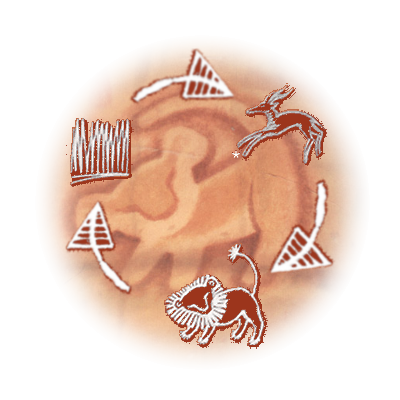
\includegraphics[scale=0.69]{images/circleEdited.png}\\
\bigskip
\LARGE{Patrick Misteli \& Ruben K{\"a}lin}

\bigskip

\bigskip

\bigskip

\bigskip

\bigskip

\bigskip

Zurich\\
May 2014\\

\end{center}



\newpage

%%%%%%%%%%%%%%%%%%%%%%%%%%%%%%%%%%%%%%%%%%%%%%%%%

\newpage
\section*{Agreement for free-download}
\bigskip


\bigskip


\large We hereby agree to make our source code for this project freely available for download from the web pages of the SOMS chair. Furthermore, we assure that all source code is written by ourselves and is not violating any copyright restrictions.

\begin{center}

\bigskip


\bigskip


\begin{tabular}{@{}p{3.3cm}@{}p{6cm}@{}@{}p{6cm}@{}}
\begin{minipage}{3cm}

\end{minipage}
&
\begin{minipage}{6cm}
\vspace{2mm} \large Patrick Misteli

 \vspace{\baselineskip}

\end{minipage}
&
\begin{minipage}{6cm}

\large Ruben K{\"a}lin

\end{minipage}
\end{tabular}


\end{center}
\newpage

%%%%%%%%%%%%%%%%%%%%%%%%%%%%%%%%%%%%%%%



% IMPORTANT
% you MUST include the ETH declaration of originality here; it is available for download on the course website or at http://www.ethz.ch/faculty/exams/plagiarism/index_EN; it can be printed as pdf and should be filled out in handwriting


%%%%%%%%%% Table of content %%%%%%%%%%%%%%%%%

\tableofcontents

\newpage

%%%%%%%%%%%%%%%%%%%%%%%%%%%%%%%%%%%%%%%



\section{Abstract}
Here lieth the abstract

\section{Individual contributions}
No clue what this is.
Maybe this?:\\ \\
Patrick: Idea + Implementation\\
Ruben: Idea polishing + performance + Math stuff

\section{Introduction and Motivations}
Intro yay

\section{Description of the Model}

\subsection{Distinction from Game of Life}
Instead of having simple cells that can either be dead or alive, the cells in our system contain organisms parametrizable using different attributes. Table \ref{tab:Properties} lists all attributes and describes their meaning.

\begin{tabular}{l|l}\label{tab:Properties}
Name & Description\\
\hline 
\hline 
Type & "Lion", "Antilope", "Grass" or "Nothing" \\ 
\hline 
PreyType & Type of the organism to prey \\ 
\hline 
Becomes & Type to become after a natural death \\ 
\hline 
FoodDigest & Amount of food digested in one day \\ 
\hline 
Stomach & Amount of food in organism \\ 
\hline 
MaxStomach & Maximal amount of food organism can contain \\ 
\hline 
DeathProb & The probability to die at the end of the day \\ 
\hline 
Fatness & The number of predator that can be fed eating the organism \\ 
\hline
Alive & 1 if alive, 0 if bitten\\
\hline 
MinStomachRepInd & Minimal amount of food needed to reproduce \\  
\hline 
RepProb & Probability to reproduce when possible\\
\hline 
IsOffspring & 1 if newborn, 0 if adult\\
\end{tabular}

\begin{tabular}{l|l}\label{tab:deathCauses}
Death Cause & Description \\ 
\hline 
\hline 
Age & The DeathProb determines if an organism dies of age at the end of each day\\ 
\hline 
Hunger & An organism with an empty stomach dies of hunger \\ 
\hline 
Eaten & Prey dies at the end of the day if bitten by predator \\  
\end{tabular} 

\section{Implementation}
We implemented a cell based system that simulates the habitat of three different species.
We compared the population results obtained form the simulation with the Lotka Volterra population curves for three species, \cite{lotkaVolterraThreeSpecies}. The results of this comparison enabled us to gain better understanding of the equilibria and the oscillating behaviour of the different populations in our simulation.
\subsection{Game of Life}

\subsection{Lotka Volterra}

$
\begin{array}{rcl}
\frac{dx}{dt} & = & ax-bxy \\ 
\frac{dy}{dt} & = & -cy+dxy-eyz \\ 
\frac{dz}{dt} & = & -fz+gyz
\end{array}
$
\section{Simulation Results and Discussion}
Death by Age $\rightarrow$ increase reproduction Rate
Cool pictures

\section{Summary and Outlook}
Answer questions

\section{References}



\bibliography{bibliography}

\end{document}  



 
